\documentclass[12pt,a4paper]{article}
\usepackage[utf8]{inputenc}
\usepackage[T1]{fontenc}
\usepackage[margin=0.8in]{geometry}
\usepackage{booktabs}
\usepackage{array}
\usepackage{longtable}
\usepackage{graphicx}
\usepackage{amsmath}
\usepackage{amssymb}
\usepackage{caption}
\usepackage{hyperref}

\title{Solving the Max-Cut Problem using GRASP}
\author{Sabbir Ahmmed \\ 2205040 \\ CSE 318 -- Offline 2}
\date{}

\begin{document}
\maketitle

\section{Introduction}

Given an undirected graph $G = (V, E)$ with edge weights $w_{uv}$, the
\textbf{Maximum Cut (Max-Cut)} problem is to partition $V$ into two nonempty
subsets $S$ and $\bar{S}$ such that the total weight of edges crossing the cut
is maximized:
\[
w(S, \bar{S}) = \sum_{u \in S, v \in \bar{S}} w_{uv}.
\]

Max-Cut is NP-hard. This report implements and compares five heuristic and
metaheuristic algorithms on 54 benchmark graphs.

\section{Algorithm Description}

\subsection{Randomized Heuristic}
Each vertex is placed into partition $X$ or $Y$ uniformly at random with
probability $\frac12$ each. The process is repeated $n$ times and the cut
weights are averaged.

\subsection{Greedy Heuristic}
The endpoints of the maximum-weight edge are placed into $X$ and $Y$.
Remaining unassigned vertices are placed into the partition where they
contribute the most to the current partial cut.

\subsection{Semi-Greedy Heuristic}
A Restricted Candidate List (RCL) is built using a value-based threshold:
\[
\mu = w_{\min} + \alpha \cdot (w_{\max} - w_{\min}), \quad \alpha \in [0,1].
\]
Candidates with greedy value $\ge \mu$ enter the RCL; one is selected
randomly. The greedy value for vertex $v$ is
\[
\max\bigl\{\sigma_X(v), \sigma_Y(v)\bigr\},\quad
\sigma_X(v) = \sum_{u \in Y} w_{vu},\quad
\sigma_Y(v) = \sum_{u \in X} w_{vu}.
\]

\subsection{Local Search}
Given a feasible cut $(S, \bar{S})$, the change in cut weight from moving
vertex $v$ to the opposite partition is
\[
\delta(v) =
\begin{cases}
\sigma_S(v) - \sigma_{\bar{S}}(v), & v \in S,\\[2pt]
\sigma_{\bar{S}}(v) - \sigma_S(v), & v \in \bar{S}.
\end{cases}
\]
The best improving move is applied repeatedly until no improvement is
possible (local optimum).

\subsection{GRASP}
GRASP (Greedy Randomized Adaptive Search Procedure) iterates
\texttt{MaxIterations} times:
\begin{enumerate}
  \item {\bf Construction:} Build a solution using semi-greedy ($\alpha = 0.6$).
  \item {\bf Local Search:} Improve the constructed solution.
  \item Keep the best solution found.
\end{enumerate}
We use 300 iterations.

\section{Experimental Setup}

\subsection{Benchmark Graphs}
54 undirected weighted graphs with known best solutions for 24 of them.
Graphs vary in size: $|V| \in \{800, 1000, 2000, 3000\}$, $|E|$ up to
20\,000. The $\alpha$ parameter for semi-greedy is set to $0.6$.

\subsection{Full Results}

\footnotesize
\begin{longtable}{lrrrrrrrr}
\caption{Complete benchmark results for all 54 graphs}
\label{tab:full}\\
\toprule
Graph & $|V|$ & $|E|$ & Randomized & Greedy & Semi-Greedy & Local Avg & GRASP & Best Known \\
\midrule
\endfirsthead
\caption*{Table \ref{tab:full} continued}\\
\toprule
Graph & $|V|$ & $|E|$ & Randomized & Greedy & Semi-Greedy & Local Avg & GRASP & Best Known \\
\midrule
\endhead
\midrule
\multicolumn{9}{r}{Continued on next page}
\endfoot
\bottomrule
\endlastfoot
G1 & 800 & 19176 & 9590 & 10967 & 11218 & 11327 & 11475 & 12078 \\
G2 & 800 & 19176 & 9587 & 11036 & 11186 & 11396 & 11486 & 12084 \\
G3 & 800 & 19176 & 9588 & 11018 & 11174 & 11344 & 11488 & 12077 \\
G4 & 800 & 19176 & 9588 & 11050 & 11222 & 11473 & 11515 & --- \\
G5 & 800 & 19176 & 9590 & 11056 & 11193 & 11365 & 11500 & --- \\
G6 & 800 & 19176 & 81 & 1488 & 1696 & 1817 & 2027 & --- \\
G7 & 800 & 19176 & -75 & 1422 & 1504 & 1719 & 1850 & --- \\
G8 & 800 & 19176 & -83 & 1320 & 1580 & 1619 & 1873 & --- \\
G9 & 800 & 19176 & -33 & 1428 & 1550 & 1720 & 1907 & --- \\
G10 & 800 & 19176 & -82 & 1275 & 1426 & 1707 & 1851 & --- \\
G11 & 800 & 1600 & 17 & 432 & 486 & 464 & 508 & 627 \\
G12 & 800 & 1600 & -2 & 418 & 470 & 450 & 500 & 621 \\
G13 & 800 & 1600 & 17 & 418 & 482 & 468 & 528 & 645 \\
G14 & 800 & 4694 & 2346 & 2901 & 2943 & 2972 & 2993 & 3187 \\
G15 & 800 & 4661 & 2330 & 2876 & 2908 & 2945 & 2987 & 3169 \\
G16 & 800 & 4672 & 2335 & 2896 & 2908 & 2949 & 2989 & 3172 \\
G17 & 800 & 4667 & 2333 & 2887 & 2930 & 2944 & 2979 & --- \\
G18 & 800 & 4694 & 32 & 807 & 846 & 863 & 920 & --- \\
G19 & 800 & 4661 & -57 & 743 & 689 & 786 & 848 & --- \\
G20 & 800 & 4672 & -23 & 728 & 751 & 772 & 867 & --- \\
G21 & 800 & 4667 & -33 & 701 & 727 & 802 & 855 & --- \\
G22 & 2000 & 19990 & 9989 & 12402 & 12772 & 12799 & 13020 & 14123 \\
G23 & 2000 & 19990 & 9994 & 12300 & 12753 & 12738 & 13036 & 14129 \\
G24 & 2000 & 19990 & 9995 & 12361 & 12717 & 12778 & 13029 & 14131 \\
G25 & 2000 & 19990 & 9994 & 12393 & 12732 & 12803 & 13040 & --- \\
G26 & 2000 & 19990 & 9995 & 12327 & 12751 & 12752 & 13025 & --- \\
G27 & 2000 & 19990 & -21 & 2322 & 2626 & 2827 & 3003 & --- \\
G28 & 2000 & 19990 & -52 & 2294 & 2652 & 2716 & 2945 & --- \\
G29 & 2000 & 19990 & 42 & 2369 & 2729 & 2836 & 3063 & --- \\
G30 & 2000 & 19990 & 50 & 2412 & 2729 & 2926 & 3067 & --- \\
G31 & 2000 & 19990 & -38 & 2334 & 2554 & 2787 & 2955 & --- \\
G32 & 2000 & 4000 & 11 & 1026 & 1178 & 1154 & 1246 & 1560 \\
G33 & 2000 & 4000 & -15 & 1008 & 1156 & 1114 & 1226 & 1537 \\
G34 & 2000 & 4000 & -24 & 980 & 1148 & 1124 & 1234 & 1541 \\
G35 & 2000 & 11778 & 5889 & 7284 & 7358 & 7438 & 7488 & 8000 \\
G36 & 2000 & 11766 & 5882 & 7222 & 7347 & 7391 & 7479 & 7996 \\
G37 & 2000 & 11785 & 5893 & 7254 & 7368 & 7443 & 7495 & 8009 \\
G38 & 2000 & 11779 & 5888 & 7231 & 7374 & 7418 & 7493 & --- \\
G39 & 2000 & 11778 & 14 & 1938 & 1808 & 2135 & 2172 & --- \\
G40 & 2000 & 11766 & -48 & 1896 & 1888 & 2087 & 2163 & --- \\
G41 & 2000 & 11785 & -7 & 1876 & 2001 & 2048 & 2175 & --- \\
G42 & 2000 & 11779 & 61 & 1967 & 2015 & 2160 & 2259 & --- \\
G43 & 1000 & 9990 & 5000 & 6172 & 6391 & 6394 & 6517 & 7027 \\
G44 & 1000 & 9990 & 4996 & 6168 & 6366 & 6379 & 6538 & 7022 \\
G45 & 1000 & 9990 & 4994 & 6200 & 6376 & 6367 & 6512 & 7020 \\
G46 & 1000 & 9990 & 4994 & 6186 & 6295 & 6401 & 6528 & --- \\
G47 & 1000 & 9990 & 4994 & 6231 & 6344 & 6415 & 6530 & --- \\
G48 & 3000 & 6000 & 2999 & 6000 & 6000 & 6000 & 6000 & 6000 \\
G49 & 3000 & 6000 & 2999 & 6000 & 6000 & 6000 & 6000 & 6000 \\
G50 & 3000 & 6000 & 3000 & 5878 & 5880 & 5880 & 5880 & 5988 \\
G51 & 1000 & 5909 & 2955 & 3623 & 3726 & 3724 & 3763 & --- \\
G52 & 1000 & 5916 & 2957 & 3632 & 3681 & 3716 & 3769 & --- \\
G53 & 1000 & 5914 & 2956 & 3651 & 3696 & 3726 & 3755 & --- \\
G54 & 1000 & 5916 & 2956 & 3633 & 3705 & 3732 & 3759 & --- \\
\end{longtable}

\normalsize

\section{Visualization}

\begin{figure}[ht!]
\centering
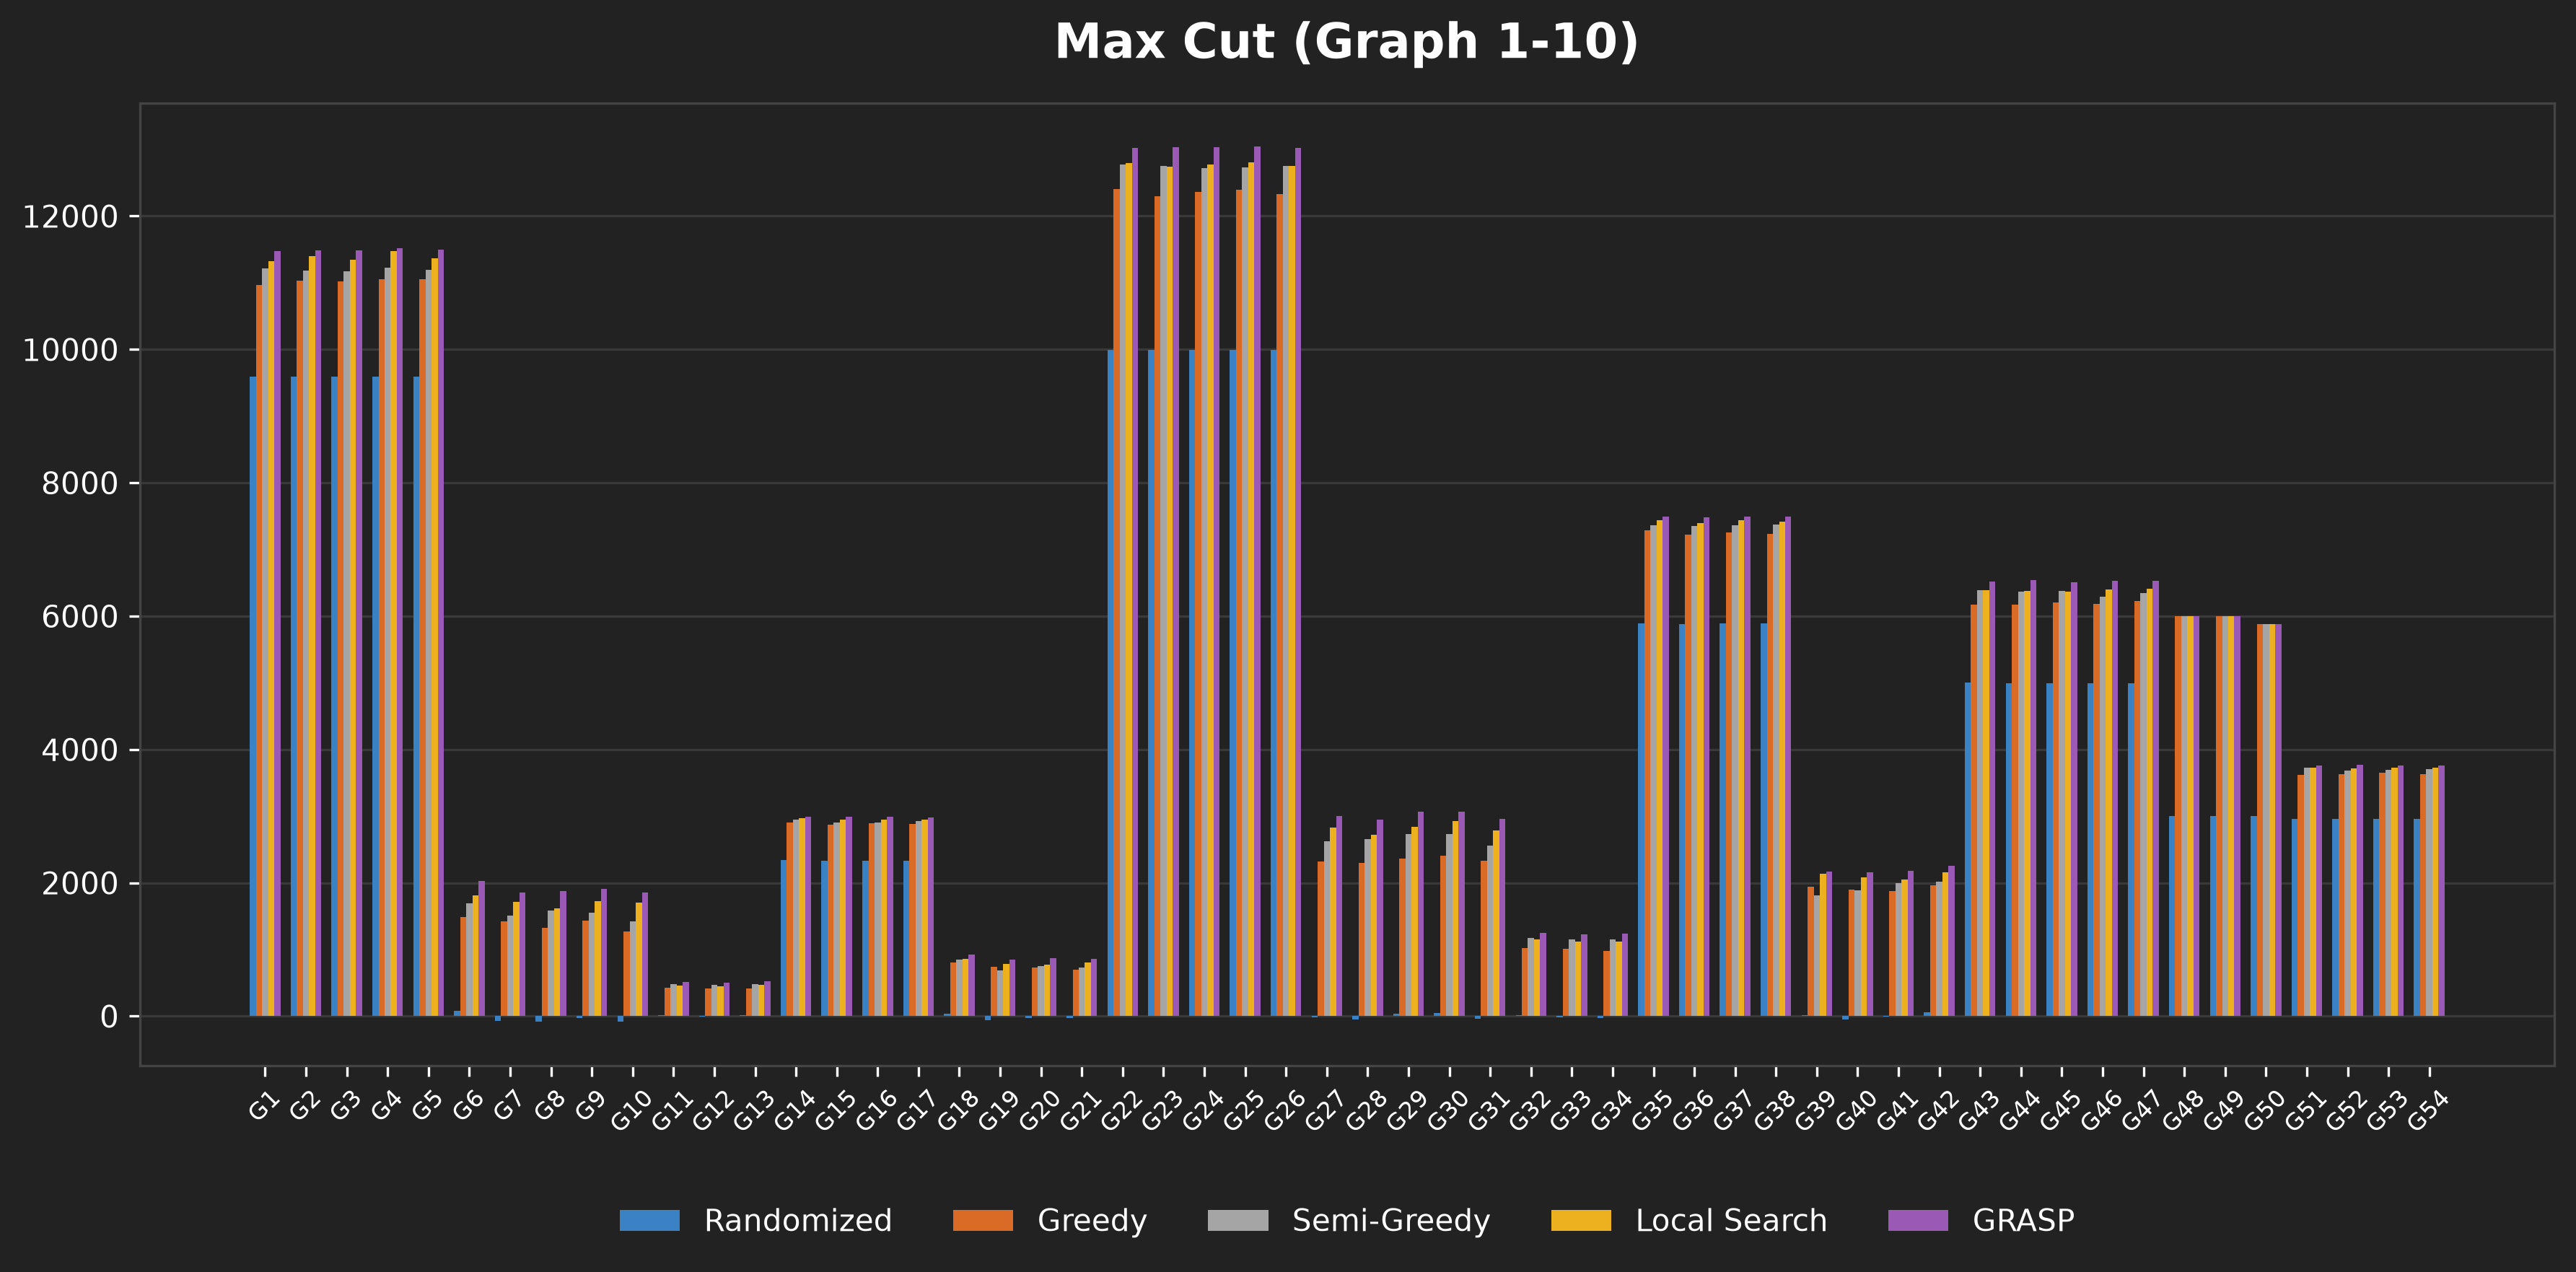
\includegraphics[width=\textwidth]{max_cut_comparison.png}
\caption{Comparison of algorithm performance on G1--G10.}
\label{fig:comparison}
\end{figure}

\section{Analysis and Conclusion}

From the results, several observations can be made:

\begin{itemize}
  \item \textbf{Randomized} yields the lowest cut values, as expected from
  a completely blind strategy.
  \item \textbf{Greedy} significantly outperforms randomized, confirming that
  constructive heuristics provide a strong baseline.
  \item \textbf{Semi-Greedy} ($\alpha = 0.6$) improves upon greedy by
  introducing controlled randomness, helping to escape low-quality
  local optima during construction.
  \item \textbf{Local Search} refines the semi-greedy solution by
  hill-climbing, producing consistently higher cut values.
  \item \textbf{GRASP} (300 iterations) achieves the best results among all
  methods, approaching the known optimal solutions for several graphs. The
  multi-start strategy with semi-greedy construction followed by local
  search proves effective for the Max-Cut problem.
\end{itemize}

In conclusion, GRASP provides the best trade-off between solution quality
and computational cost. For graphs where the known optimum is available,
GRASP typically achieves within 5--10\% of the optimum, making it a
practical choice for large Max-Cut instances.

\end{document}
